In this section we present the implementation details of {\em RambutanAcc}.
At the high level, the runtime is constituted of 3 major modules: task management system, communication handler, and task scheduler as shown in Fig.~\ref{fig:impl}. 
The runtime can be configured to run on a dedicated processor core in order to keep it responsive.

\begin{figure}[htb]
\centering
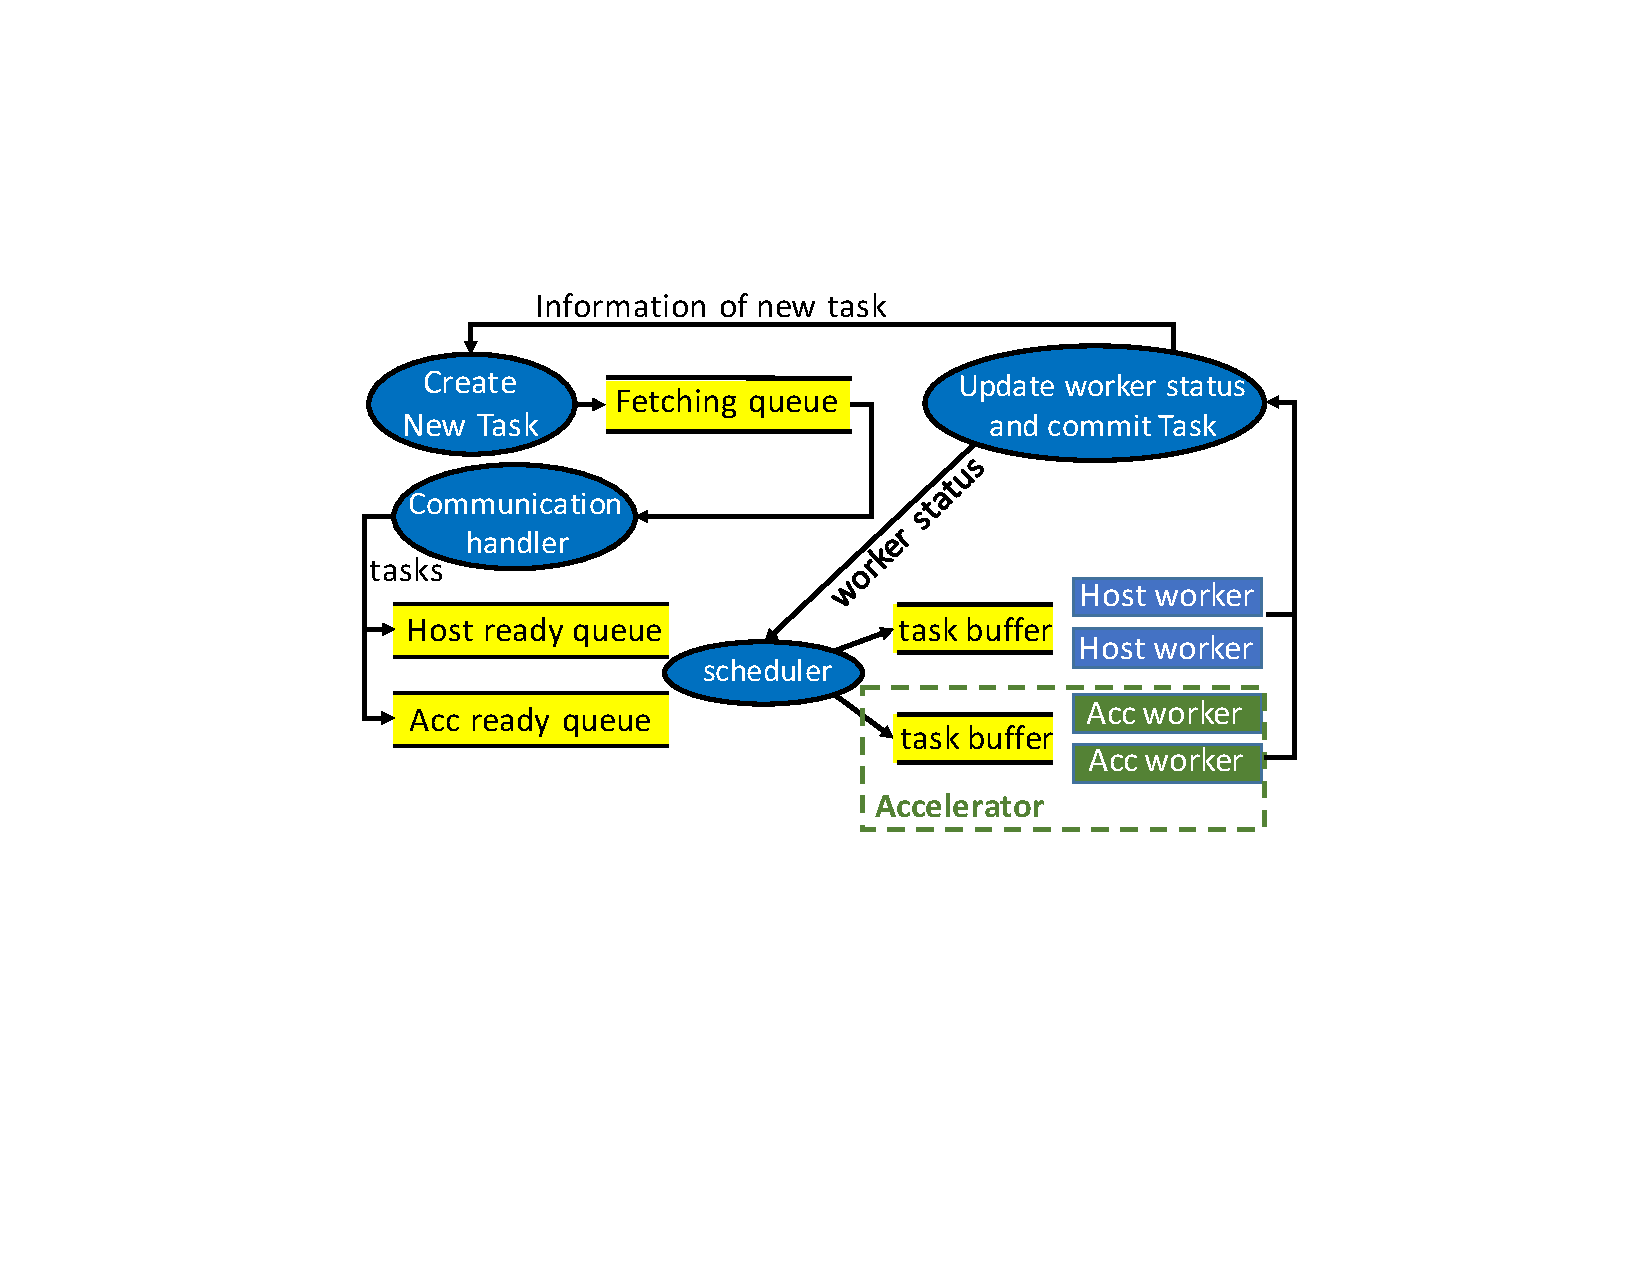
\includegraphics[width=.49\textwidth]{figures/impl.pdf}
\caption{Runtime implementation}
\label{fig:impl}
\end{figure}

\subsection{Task Management System}
Tasks can be created as soon as input data are produced.
The task management system listens for requests from existing tasks to create new tasks.
A task may own data.
Upon the completion of a task, the task management system may write data back (if necessary) before destroying the task.
If the task executed on accelerator while original data resides in host memory, data will be written back to host asynchronously, overlapping with other tasks' computations.
If original data locate in a different place, the task management system asks the communication handlers to write data back.

\subsection{Communication handlers}
Once a task has been created, it will be pushed to the {\em fetching queue} by the task management system.
The communication handler periodically pulls tasks from this queue and fetches their input data.
Depending on the available memory resource, a certain number of tasks in the {\em fetching queue} will be served at a time.
{\em RambutanAcc} supports both on-node and off-node communication.

Within a single node, we use communication primitives provided by the accelerator's vendor.
In particular, on compute nodes with NVIDIA's GPUs, we use CUDA stream to move data between host and GPUs.
On Intel's KNC based nodes, we use COI (Coprocessor Offload Infrastructure).
To avoid blocking the runtime, we don't use any synchronization routine.
Instead, the communication handler periodically tests the completion of communication activities.

We employ GASNet to implement the off-node communication handler.
The process of fetching data from a remote node is shown in Fig.~\ref{fig:offnode}.
To fetch remote data for a task, the corresponding GASNet process issues a remote procedural call to request data from the process that holds the task owning the data (1).
This procedure looks for the appropriate data at the remote node.
If data resides in accelerator memory, the remote procedure has also to pull data up before sending data (2).
Once the memory transfer from accelerator completes (3), data can be sent to the requester using the one-sided {\em put} operation (4).
Once the remote GASNet process finishes the remote data transfer, it issues a response remote procedural call to push data to the accelerator of the requester (if necessary) and notify the requester when data is available for the task.
All these activities run asynchronously and we use a polling mechanism to avoid blocking the runtime.
The process of writing data back is similar to the fetching process, and it is also handled asynchronously.


\begin{figure}[htb]
\centering
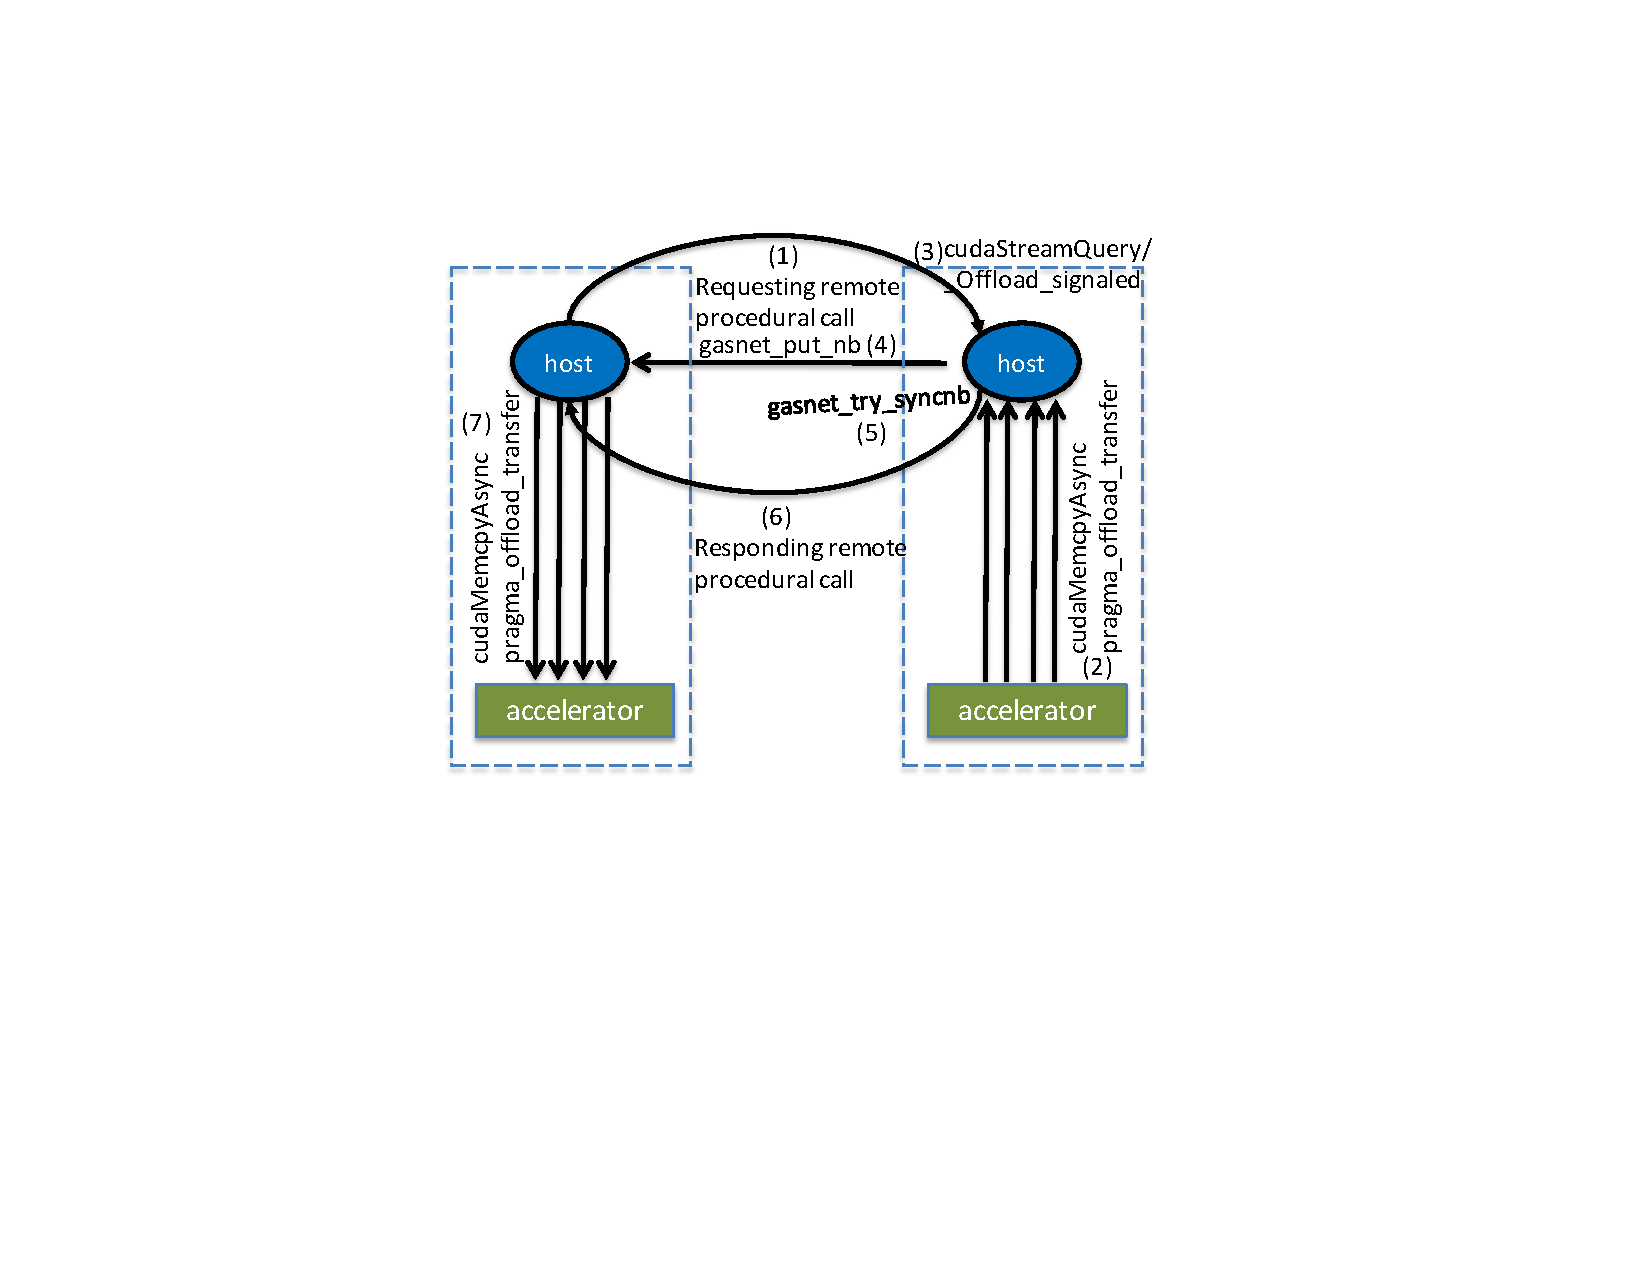
\includegraphics[width=.49\textwidth]{figures/handler.pdf}
\caption{Implementation of the off-node communication handler}
\label{fig:offnode}
\end{figure}

\subsection{Task Scheduler}
Tasks become {\em ready} and pushed in the {\em ready queues} once all of their data have been fetched.
Each GASNet process runs a task scheduler to dispatch {\em ready tasks} to workers. 

\subsubsection{Task Buffer}
To keep workers busy, the scheduler frequently checks the runnable task queue and the status of workers.
However, the task scheduler may not be very responsive since the communication handlers also run on the same processor core.
Thus, each worker has a task buffer with a few slots.
The scheduler fills up these slots while the workers keep popping tasks and execute.
To reduce synchronization overheads we use a lock-free implementation for this single producer-multiple consumers scheme.

\subsubsection{Acc worker using CUDA persistent kernel}
Since the host worker implementation is simple, we now just present the implementation of accelerator workers on GPUs.
A {\em RambutanAcc} program just launches a CUDA kernel to set up workers on GPUs' SMs and execute assigned tasks.
Once the kernel is launched, CUDA thread blocks find out what SM they are mapped to by the CUDA runtime.
Getting this information is possible by inserting PTX code to read a special register that holds SM ID.
As shown in Fig.~\ref{fig:kernel}, we keep only a certain number of thread blocks per SM (this number can be set via an environment variable and the default value is 1).
The reason is that thread blocks run until the program completes and CUDA runtime co-runs only a limited number of thread blocks on the same SM.
The alive thread blocks will be divided into workers.
Each worker is a group of threads blocks, acting as the new CUDA grid for scheduled tasks.

\begin{figure}[htb]
\centering
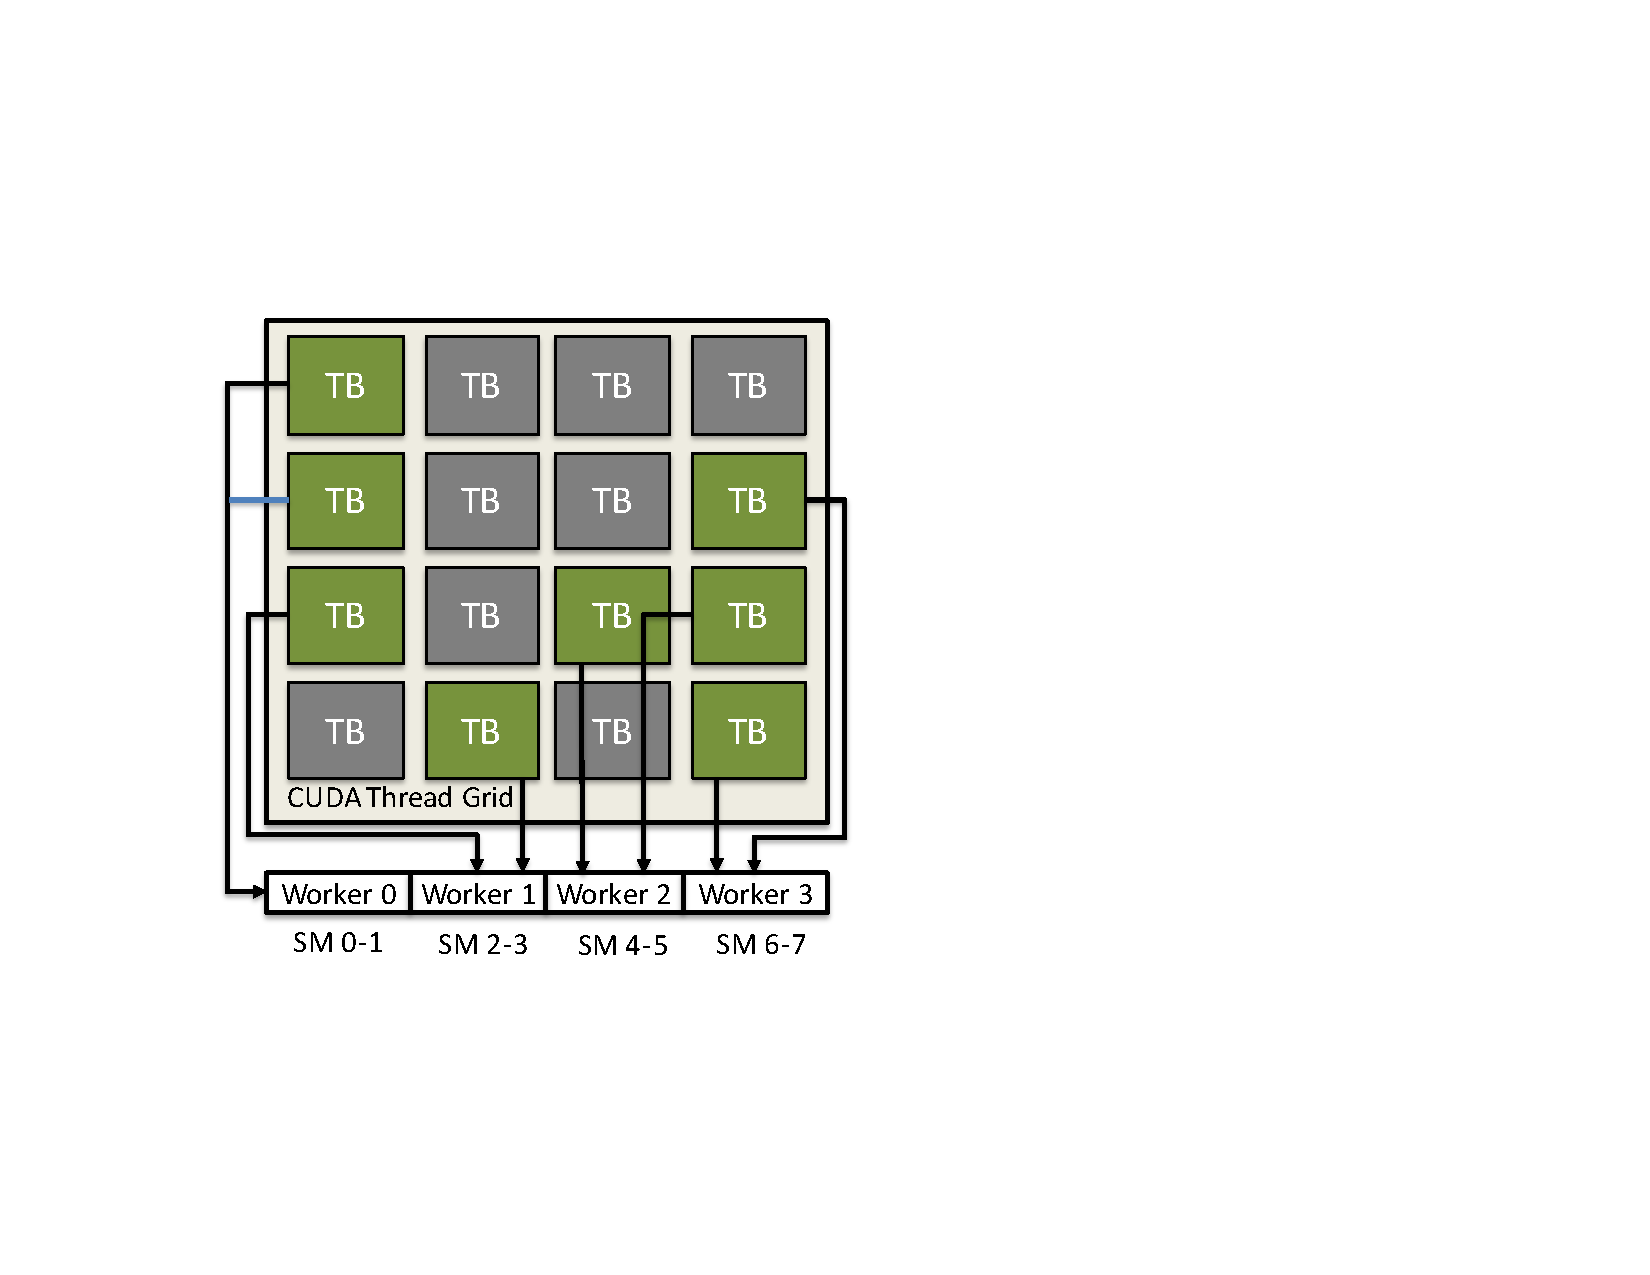
\includegraphics[width=.35\textwidth]{figures/kernel_init.pdf}
\caption{The persistent kernel selects only a limited number of thread blocks per SM (green color). The default number of thread blocks per SM is 1. 
The alive thread blocks are divided into workers to execute tasks.}
\label{fig:kernel}
\end{figure}

Now each thread block knows which worker it belongs to and where to find tasks to execute.
Once there are ready tasks and an available worker slot, the scheduler offloads corresponding function and arguments to task buffers on the GPUs.
Then the scheduler picks a worker and notifies it by writing a signal to the GPU using the nonblocking copy {\em cudaMemcpyCpyAsync}.
If the worker is busy at the time, it will read the signal  and execute the corresponding task later.
Once the task finishes, the worker notifies the scheduler.
Since a CUDA kernel cannot send data to the host, we have to use UVM (unified virtual memory).

